\documentclass[10pt,a4paper,titlepage]{jreport} % ドキュメントクラスを1つに統一


\usepackage[top=25truemm,bottom=25truemm,left=20truemm,right=20truemm]{geometry} % 余白設定
\usepackage[dvipdfmx]{graphicx} % 画像の挿入
\usepackage{graphicx}
\usepackage{listings} % コードリスト用
\usepackage{jlisting} % 日本語対応のリスト用
\usepackage{jverb} % 日本語のベタ打ち
\usepackage{booktabs}
\usepackage{pgfplots} % グラフ描画用パッケージ
\pgfplotsset{compat=1.18} % バージョン指定
\usepackage{float}
\parindent = 0pt % 段落の字下げを無効化

\usepackage{titlesec}
\usepackage{etoolbox}
\makeatletter
\patchcmd{\chapter}{\if@openleft\cleardoublepage\else\if@openright\cleardoublepage\else\clearpage\fi\fi}{}{}{}
\makeatother
\lstset{breaklines=true, postbreak=\mbox{$\hookrightarrow$}\space, keepspaces=true, escapeinside={\%*}{*)}}

\titleformat{\chapter}[hang] % 章のフォーマットを変更
  {\normalfont\huge\bfseries} % フォント設定
  {\thechapter} % 番号部分の表示形式
  {1em} % 番号とタイトルの間のスペース
  {} % タイトルの前に入れる内容（ここでは空）
\usepackage{xcolor}
\usepackage{amsmath}
\usepackage{amssymb} % ←これで \mathbb{R} が使える

\lstset{
  language=Matlab,              % 言語はMATLAB
  basicstyle=\ttfamily\small,   % フォントは等幅、サイズ小さめ
  keywordstyle=\color{blue},    % キーワード（function, endとか）を青
  commentstyle=\color{green!50!black}, % コメントを深緑
  stringstyle=\color{red!70!black},    % 文字列（'...'）を赤系
  numbers=left,                 % 行番号を左に表示
  numberstyle=\tiny\color{gray},% 行番号をグレーで小さく
  stepnumber=1,                 % 毎行行番号つける
  numbersep=10pt,               % コードとの間隔
  backgroundcolor=\color{gray!10}, % 背景うっすらグレー
  frame=single,                 % 枠をつける
  rulecolor=\color{black},      % 枠線は黒
  breaklines=true,              % 長い行を折り返す
  breakatwhitespace=false,      % スペースでだけ折り返すか（falseにして自然な折り返し）
  showspaces=false,             % スペースは特別に表示しない
  showstringspaces=false,       % 文字列中のスペースも普通に表示
  tabsize=2                     % タブ幅2
}


\title{システム制御コンピューティング　第2回レポート} % タイトル
\author{
  学生番号：242C2016  氏名：奥村直 \\
  \\
  知的システム工学科システム制御コース
  } % 著者
\date{\today} % 日付

\begin{document}

\maketitle

\chapter{課題02-1}

\section{作成したブロック線図の画像を提出しなさい。}

\begin{figure}[H]
  \centering
  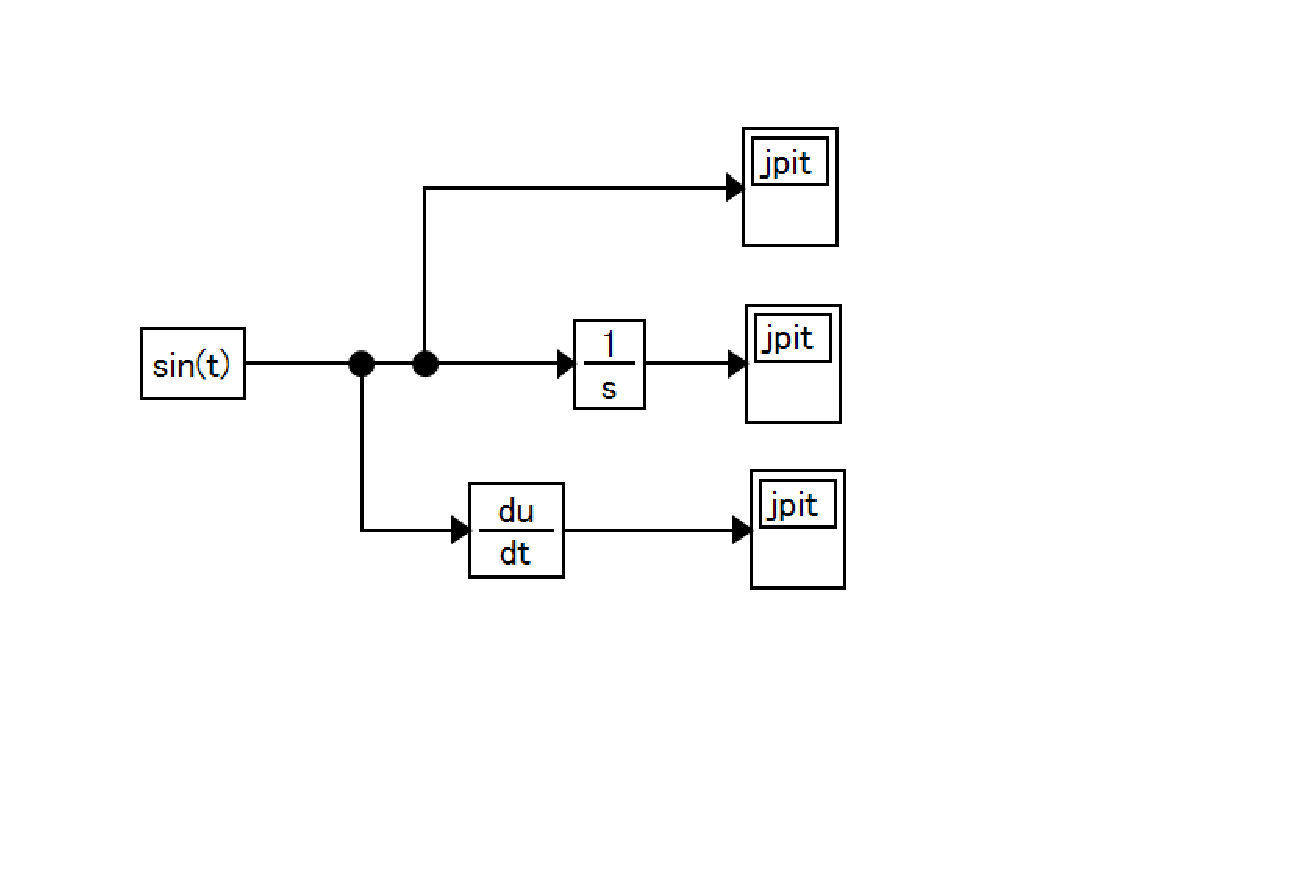
\includegraphics[width=0.8\linewidth]{circuit1.eps}
  \caption{（A）ブロック線図}
  \label{fig:sample}
\end{figure}

\section{観察された信号のグラフを提出しなさい。}

\begin{figure}[H]
  \centering
  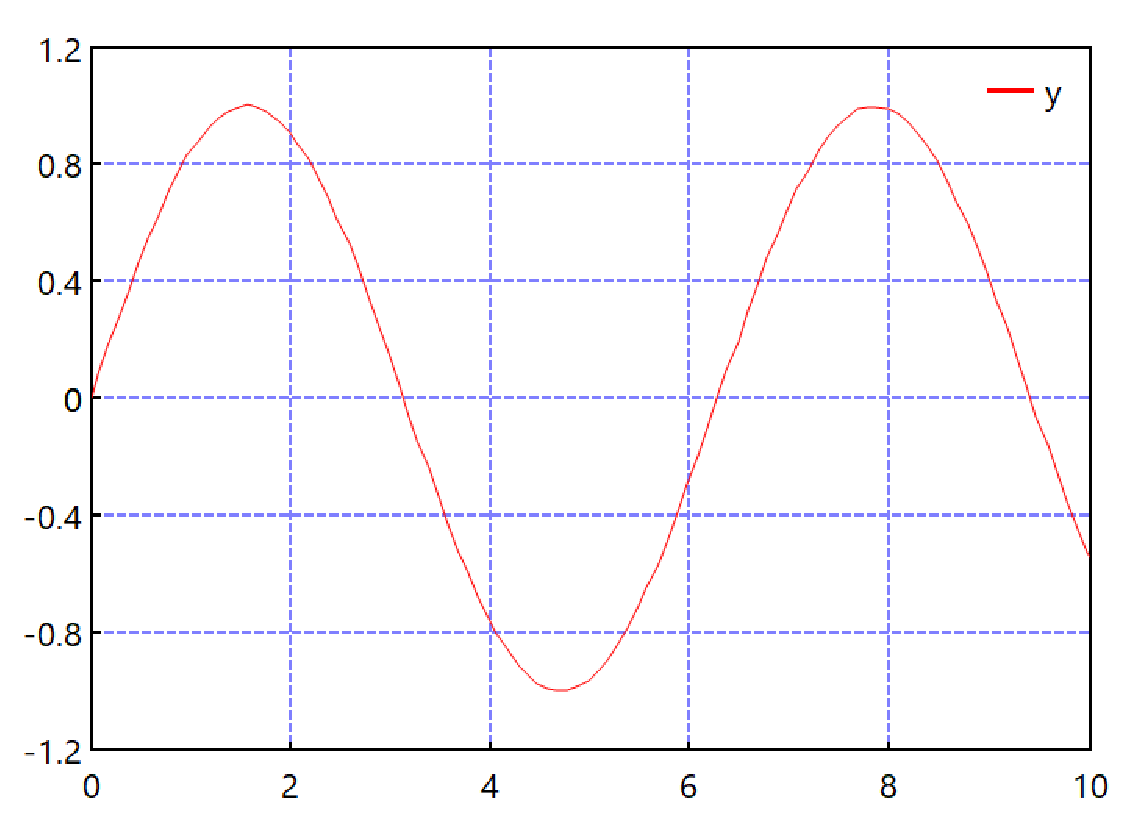
\includegraphics[width=0.8\linewidth]{sin.eps}
  \caption{（A）正弦波}
  \label{fig:sample1}
\end{figure}

\begin{figure}[H]
  \centering
  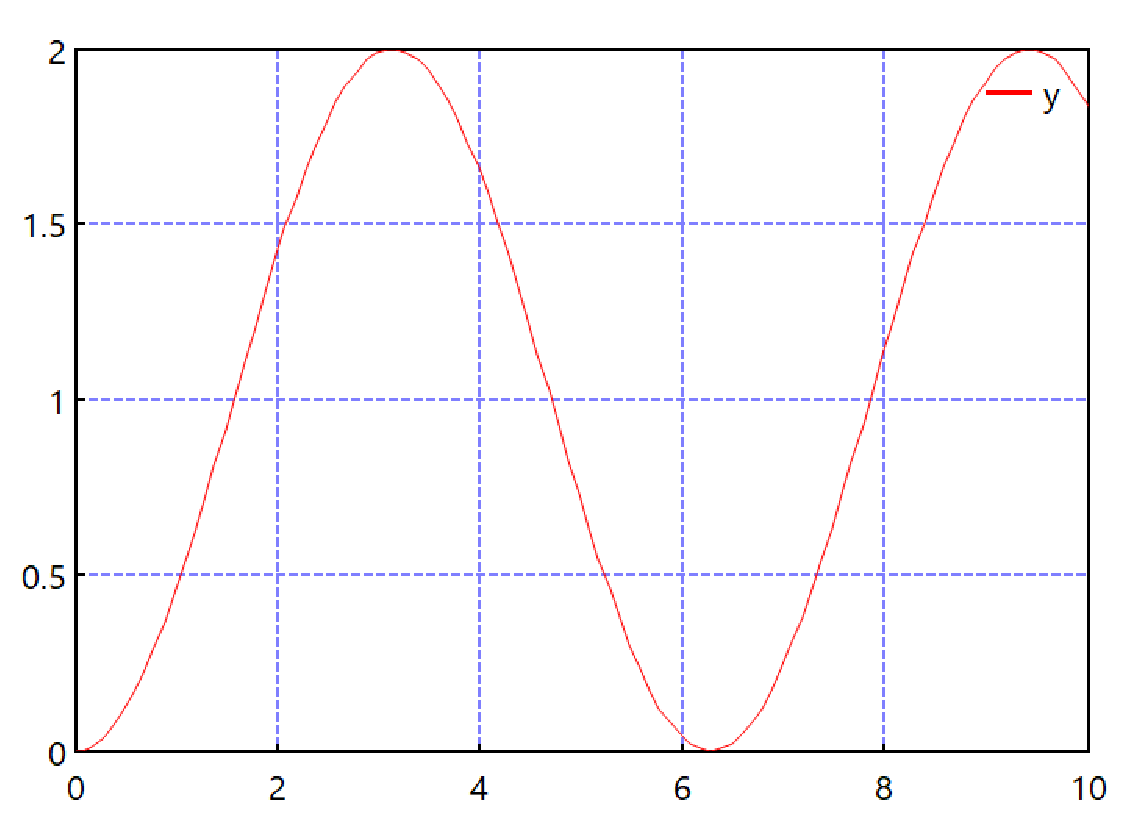
\includegraphics[width=0.8\linewidth]{differential.eps}
  \caption{（B）積分器}
  \label{fig:sample2}
\end{figure}

\begin{figure}[H]
  \centering
  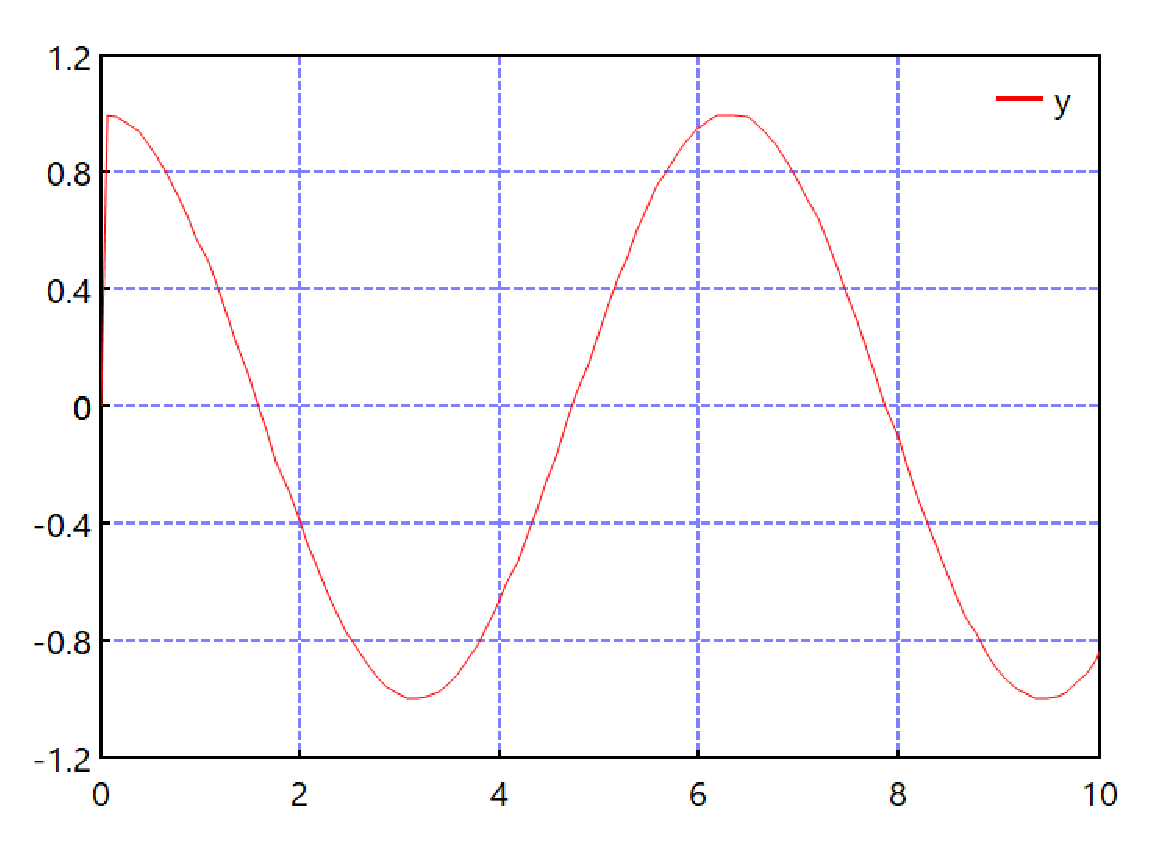
\includegraphics[width=0.8\linewidth]{integral.eps}
  \caption{（C）微分器（差分近似）}
  \label{fig:sample3}
\end{figure}

\section{システムの入出力特性について考察しなさい。（なぜ、そのような信号が観察されたか）}

（A）は、グラフの波形を見ると $ y = \sin(t)$ であると分かる。

$\sin(t)$ の積分と微分を考えると、 \\
積分をした場合、

\begin{equation}
\int \sin(t) dt = -\cos(t) + C （Cは積分定数）
\end{equation}

つまり、余弦波となり正弦波に対して $\frac{\pi}{2}$ の遅れ位相となる。
したがって積分後の符号も考慮すると、 $y = \int \sin(t)$ であると分かる。 
また、振幅が0~2となっている理由としては、初期値Cが考えられる。初期値Cは式とグラフより1であったと推測できる。

次に微分をした場合、

\begin{equation}
\frac{d}{dt} sin(t) = \cos(t)
\end{equation}

つまり、余弦はとなり正弦波に対して $\frac{\pi}{2}$ の進み位相となる。
したがって積分後の符号も考慮すると、$y = \frac{d}{dt} sin(t)$ であると分かる。

これらの結果から分かるシステムの入出力特性を考察すると、微分器を使用するときは定数のことを考慮する必要はないが、
積分器を使用する場合、不定積分が行われるため、演算後に生じる積分定数のことを考慮しなければグラフの振幅に変化をもたらしてしまうことが分かる。

余談だが、位相の遅れと進みは変数tの係数を考慮すると簡単に考えることができる。

\end{document}
